% --- [ Recovery of N-way Conditionals ] ---------------------------------------

\subsection{Recovery of N-way Conditionals}
\label{sec:recovery_of_nway_conditionals}

The control flow recovery results of the Hammock method, the Interval method, and for comparison the theoretical optimum when recovering \textit{n-way conditionals} (e.g. \texttt{switch}-statements) from the combined test programs of Coreutils and SQLite are presented in figure \ref{fig:total_results_nway}.

The \textbf{Hammock method} correctly recovered $0.00\%$ of the n-way conditionals present in the test programs (\textit{true positives}). On average, for every $10$ n-way conditionals of the original source code, the Hammock method recovered $0.0$ n-way conditionals that were \textit{not} present of the original source code (\textit{false positives}).

The \textbf{Interval method} correctly recovered $73.40\%$ of the n-way conditionals present in the test programs (\textit{true positives}). On average, for every $10$ n-way conditionals of the original source code, the Interval method recovered $19.7$ n-way conditionals that were \textit{not} present of the original source code (\textit{false positives}).

\begin{figure}[htbp]
	\centering
	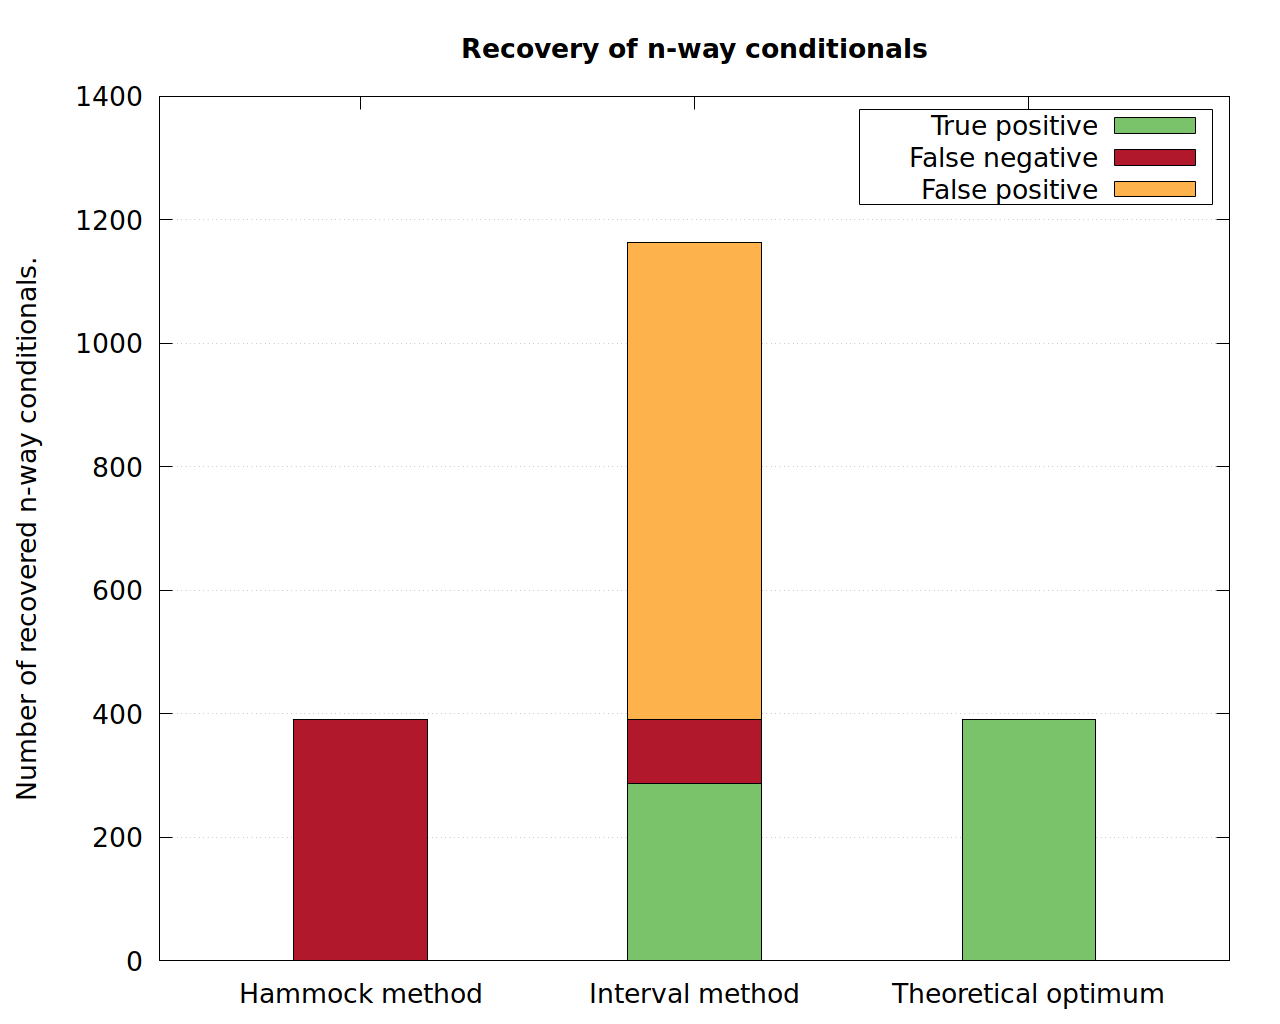
\includegraphics[width=\textwidth]{inc/5_results/results_n-way.png}
	\caption{Comparison of control flow recovery results for each method when recovering \textit{n-way conditionals}. The data is based on the combined test programs of Coreutils and SQLite.}
	\label{fig:total_results_nway}
\end{figure}
